\def \hmina {\hspace{-0.1in}}
\def \hminb {\hspace{-0.2in}}

\def \fgw {2in}
\def \fgh {1in}

% \begin{floatingfigure}[r]{2in}  (and \end{..})

\begin{figure}[t]
    \centerline{
        % \hmina
        {\begin{tikzpicture}[baseline]

    \pgfmathsetmacro{\ymax}{1.1} % set the maximum y value
    \pgfmathsetmacro{\ymaxbreak}{1.2} % set the y value at which overflow is drawn

    \begin{groupplot}[
        group style={
            group size=2 by 2,
            xlabels at=edge bottom,
            ylabels at=edge left,
            xticklabels at=edge bottom,
            yticklabels at=edge left,
            vertical sep=25pt,
            horizontal sep=15pt,
        },
        %axis x line*=bottom,
        height=3cm,
        width=\textwidth/4,
        tick align=outside,
        tick pos=bottom, % make sure ticks only appear at the bottom and left axes
        title style={yshift=-1.0ex},
        tick style={ black },
        y tick label style={ /pgf/number format/fixed, /pgf/number format/precision=0 },
        grid style={ dotted, gray },
        scatter,
        point meta=explicit symbolic,
        scatter/classes={
            c8={mark=square*},
            c20={mark=triangle*},
            ff={mark=diamond*},
            fb={mark=pentagon*},
            fs={mark=*},
            mirrored={mark=otimes},
            selective={mark=oplus}
        },
        %every node near coord/.append style={font=\tiny},
        %
        % magic to make the numbers appear above the overly long bars:
        % visualization depends on={rawy \as \rawy}, % save original y values
        % restrict y to domain*={ % now clip/restrict any y value to ymax
        %     \pgfkeysvalueof{/pgfplots/ymin}:\ymaxbreak
        % },
        % after end axis/.code={ % draw squiggly line indicating break
        %     \draw [semithick, white, decoration={snake,amplitude=0.1mm,segment length=0.75mm,post length=0.375mm}, decorate] (rel axis cs:0,1.01) -- (rel axis cs:1,1.01);
        % },
        % nodes near coords={\color{.!75!black}\pgfmathprintnumber\rawy}, % print the original y values (darkened in case they are too light)...
        % nodes near coords greater equal only=\ymax, % ... but ONLY if they are >= ymax
        clip=false, % allow clip to protrude beyond ymax
        % Custom stuff to edit per template
        %
        xlabel near ticks,
        %xlabel shift={-5mm},
        xmin=0, xmax=4,
        %%major x tick style=transparent,
        %enlarge x limits=0.2, % add some breathing room along the x axis's sides
        %
        ylabel={\scriptsize Latency (norm)},
        ylabel near ticks,
        %label shift={-1.5mm},
        ymajorgrids=true,
        ymin=0, ymax=\ymax,
        ytick={ 0, 1, \ymax },
        yticklabels={ 0, 1, \empty },
        %yticklabels={ 0, 0.5, 1.5, 2 },
        % extra y ticks={1},
        % extra y tick style={grid=major, grid style={dashed, black}},
        % extra y tick label={\empty},
        %bar width=4.5pt, % change size of bars
        %
        legend cell align=left,
        legend style={ column sep=1ex },
        legend entries={
            {\scriptsize Baseline},
            {\scriptsize Mirrored},
            {\scriptsize Selective},
            {\scriptsize },
            {\scriptsize },
            {\scriptsize C8},
            {\scriptsize C20},
            {\scriptsize FF},
            {\scriptsize FB},
            {\scriptsize FS}
        },
        legend style={
            draw=none,
            legend columns=5,
            at={(1.0,1.45)},
            anchor=south,
        },
    ]
        \nextgroupplot[title={\footnotesize 40M Mirrored Reads}]
            \addlegendimage{mark=none,red}
            \addlegendimage{mark=otimes,only marks,black}
            \addlegendimage{mark=oplus,only marks,black}
            \addlegendimage{only marks,mark=square*,white}
            \addlegendimage{only marks,mark=square*,white}
            \addlegendimage{only marks,mark=square*,red}
            \addlegendimage{only marks,mark=triangle*,red}
            \addlegendimage{only marks,mark=diamond*,red}
            \addlegendimage{only marks,mark=pentagon*,red}
            \addlegendimage{only marks,mark=*,red}
            \addplot [thick, red] table [
                meta=cipher,
                x=score,
                y=latency,
                discard if symbol not={iop}{40m-r},
                discard if symbol not={ratio}{0},
                discard if symbol not={strategy}{mirrored},
                col sep=space,
            ] {data/tradeoff-ms.dat};
            \addplot [only marks] table [
                meta=strategy,
                x=score,
                y=latency,
                discard if symbol not={iop}{40m-r},
                discard if symbol not={ratio}{1},
                discard if symbol not={strategy}{mirrored},
                col sep=space
            ] {data/tradeoff-ms.dat};
            \addplot [only marks] table [
                meta=strategy,
                x=score,
                y=latency,
                discard if symbol not={iop}{40m-r},
                discard if symbol not={ratio}{2},
                discard if symbol not={strategy}{mirrored},
                col sep=space
            ] {data/tradeoff-ms.dat};
            \addplot [only marks] table [
                meta=strategy,
                x=score,
                y=latency,
                discard if symbol not={iop}{40m-r},
                discard if symbol not={ratio}{3},
                discard if symbol not={strategy}{mirrored},
                col sep=space
            ] {data/tradeoff-ms.dat};
        \nextgroupplot[
            legend to name={throwaway15},
            title={\footnotesize 40M Mirrored Writes}
        ]
            \addplot [thick, red] table [
                meta=cipher,
                x=score,
                y=latency,
                discard if symbol not={iop}{40m-w},
                discard if symbol not={ratio}{0},
                discard if symbol not={strategy}{mirrored},
                col sep=space,
            ] {data/tradeoff-ms.dat};
            \addplot [only marks] table [
                meta=strategy,
                x=score,
                y=latency,
                discard if symbol not={iop}{40m-w},
                discard if symbol not={ratio}{1},
                discard if symbol not={strategy}{mirrored},
                col sep=space
            ] {data/tradeoff-ms.dat};
            \addplot [only marks] table [
                meta=strategy,
                x=score,
                y=latency,
                discard if symbol not={iop}{40m-w},
                discard if symbol not={ratio}{2},
                discard if symbol not={strategy}{mirrored},
                col sep=space
            ] {data/tradeoff-ms.dat};
            \addplot [only marks] table [
                meta=strategy,
                x=score,
                y=latency,
                discard if symbol not={iop}{40m-w},
                discard if symbol not={ratio}{3},
                discard if symbol not={strategy}{mirrored},
                col sep=space
            ] {data/tradeoff-ms.dat};
        % \nextgroupplot[legend to name={throwaway20}, title={\footnotesize 4K Mirrored Reads}]
        %     \addplot [thick, red] table [
        %         meta=cipher,
        %         x=score,
        %         y=latency,
        %         discard if symbol not={iop}{4k-r},
        %         discard if symbol not={ratio}{0},
        %         discard if symbol not={strategy}{mirrored},
        %         col sep=space,
        %     ] {data/tradeoff-ms.dat};
        %     \addplot [only marks] table [
        %         meta=strategy,
        %         x=score,
        %         y=latency,
        %         discard if symbol not={iop}{4k-r},
        %         discard if symbol not={ratio}{1},
        %         discard if symbol not={strategy}{mirrored},
        %         col sep=space
        %     ] {data/tradeoff-ms.dat};
        %     \addplot [only marks] table [
        %         meta=strategy,
        %         x=score,
        %         y=latency,
        %         discard if symbol not={iop}{4k-r},
        %         discard if symbol not={ratio}{2},
        %         discard if symbol not={strategy}{mirrored},
        %         col sep=space
        %     ] {data/tradeoff-ms.dat};
        %     \addplot [only marks] table [
        %         meta=strategy,
        %         x=score,
        %         y=latency,
        %         discard if symbol not={iop}{4k-r},
        %         discard if symbol not={ratio}{3},
        %         discard if symbol not={strategy}{mirrored},
        %         col sep=space
        %     ] {data/tradeoff-ms.dat};
        % \nextgroupplot[legend to name={throwaway14}, title={\footnotesize 4K Selective Reads}]
        %     \addplot [thick, red] table [
        %         meta=cipher,
        %         x=score,
        %         y=latency,
        %         discard if symbol not={iop}{4k-r},
        %         discard if symbol not={ratio}{0},
        %         discard if symbol not={strategy}{selective},
        %         col sep=space,
        %     ] {data/tradeoff-ms.dat};
        %     \addplot [only marks] table [
        %         meta=strategy,
        %         x=score,
        %         y=latency,
        %         discard if symbol not={iop}{4k-r},
        %         discard if symbol not={ratio}{1},
        %         discard if symbol not={strategy}{selective},
        %         col sep=space
        %     ] {data/tradeoff-ms.dat};
        %     \addplot [only marks] table [
        %         meta=strategy,
        %         x=score,
        %         y=latency,
        %         discard if symbol not={iop}{4k-r},
        %         discard if symbol not={ratio}{2},
        %         discard if symbol not={strategy}{selective},
        %         col sep=space
        %     ] {data/tradeoff-ms.dat};
        %     \addplot [only marks] table [
        %         meta=strategy,
        %         x=score,
        %         y=latency,
        %         discard if symbol not={iop}{4k-r},
        %         discard if symbol not={ratio}{3},
        %         discard if symbol not={strategy}{selective},
        %         col sep=space
        %     ] {data/tradeoff-ms.dat};
        \nextgroupplot[
            legend to name={throwaway19},
            title={\footnotesize 40M Selective Reads},
            xlabel={\scriptsize Trade Score},
            xtick={ 0, 1, 2, 3, 4 },
            xticklabels={ 0,,, 1, \empty }
        ]
            \addplot [thick, red] table [
                meta=cipher,
                x=score,
                y=latency,
                discard if symbol not={iop}{40m-r},
                discard if symbol not={ratio}{0},
                discard if symbol not={strategy}{selective},
                col sep=space,
            ] {data/tradeoff-ms.dat};
            \addplot [only marks] table [
                meta=strategy,
                x=score,
                y=latency,
                discard if symbol not={iop}{40m-r},
                discard if symbol not={ratio}{1},
                discard if symbol not={strategy}{selective},
                col sep=space
            ] {data/tradeoff-ms.dat};
            \addplot [only marks] table [
                meta=strategy,
                x=score,
                y=latency,
                discard if symbol not={iop}{40m-r},
                discard if symbol not={ratio}{2},
                discard if symbol not={strategy}{selective},
                col sep=space
            ] {data/tradeoff-ms.dat};
            \addplot [only marks] table [
                meta=strategy,
                x=score,
                y=latency,
                discard if symbol not={iop}{40m-r},
                discard if symbol not={ratio}{3},
                discard if symbol not={strategy}{selective},
                col sep=space
            ] {data/tradeoff-ms.dat};
        \nextgroupplot[
            legend to name={throwaway16},
            title={\footnotesize 40M Selective Writes},
            xlabel={\scriptsize Trade Score},
            xtick={ 0, 1, 2, 3, 4 },
            xticklabels={ 0,,, 1, \empty }
        ]
            \addplot [thick, red] table [
                meta=cipher,
                x=score,
                y=latency,
                discard if symbol not={iop}{40m-w},
                discard if symbol not={ratio}{0},
                discard if symbol not={strategy}{selective},
                col sep=space,
            ] {data/tradeoff-ms.dat};
            \addplot [only marks] table [
                meta=strategy,
                x=score,
                y=latency,
                discard if symbol not={iop}{40m-w},
                discard if symbol not={ratio}{1},
                discard if symbol not={strategy}{selective},
                col sep=space
            ] {data/tradeoff-ms.dat};
            \addplot [only marks] table [
                meta=strategy,
                x=score,
                y=latency,
                discard if symbol not={iop}{40m-w},
                discard if symbol not={ratio}{2},
                discard if symbol not={strategy}{selective},
                col sep=space
            ] {data/tradeoff-ms.dat};
            \addplot [only marks] table [
                meta=strategy,
                x=score,
                y=latency,
                discard if symbol not={iop}{40m-w},
                discard if symbol not={ratio}{3},
                discard if symbol not={strategy}{selective},
                col sep=space
            ] {data/tradeoff-ms.dat};
        % \nextgroupplot[
        %     legend to name={throwaway17},
        %     title={\footnotesize 4K Mirrored Writes},
        %     xlabel={\scriptsize Trade Score},
        %     xtick={ 0, 1, 2, 3, 4 },
        %     xticklabels={ 0,,, 1, \empty }
        % ]
        %     \addplot [thick, red] table [
        %         meta=cipher,
        %         x=score,
        %         y=latency,
        %         discard if symbol not={iop}{4k-w},
        %         discard if symbol not={ratio}{0},
        %         discard if symbol not={strategy}{mirrored},
        %         col sep=space,
        %     ] {data/tradeoff-ms.dat};
        %     \addplot [only marks] table [
        %         meta=strategy,
        %         x=score,
        %         y=latency,
        %         discard if symbol not={iop}{4k-w},
        %         discard if symbol not={ratio}{1},
        %         discard if symbol not={strategy}{mirrored},
        %         col sep=space
        %     ] {data/tradeoff-ms.dat};
        %     \addplot [only marks] table [
        %         meta=strategy,
        %         x=score,
        %         y=latency,
        %         discard if symbol not={iop}{4k-w},
        %         discard if symbol not={ratio}{2},
        %         discard if symbol not={strategy}{mirrored},
        %         col sep=space
        %     ] {data/tradeoff-ms.dat};
        %     \addplot [only marks] table [
        %         meta=strategy,
        %         x=score,
        %         y=latency,
        %         discard if symbol not={iop}{4k-w},
        %         discard if symbol not={ratio}{3},
        %         discard if symbol not={strategy}{mirrored},
        %         col sep=space
        %     ] {data/tradeoff-ms.dat};
        % \nextgroupplot[
        %     legend to name={throwaway18},
        %     title={\footnotesize 4K Selective Writes},
        %     xlabel={\scriptsize Trade Score},
        %     xtick={ 0, 1, 2, 3, 4 },
        %     xticklabels={ 0,,, 1, \empty }
        % ]
        %     \addplot [thick, red] table [
        %         meta=cipher,
        %         x=score,
        %         y=latency,
        %         discard if symbol not={iop}{4k-w},
        %         discard if symbol not={ratio}{0},
        %         discard if symbol not={strategy}{selective},
        %         col sep=space,
        %     ] {data/tradeoff-ms.dat};
        %     \addplot [only marks] table [
        %         meta=strategy,
        %         x=score,
        %         y=latency,
        %         discard if symbol not={iop}{4k-w},
        %         discard if symbol not={ratio}{1},
        %         discard if symbol not={strategy}{selective},
        %         col sep=space
        %     ] {data/tradeoff-ms.dat};
        %     \addplot [only marks] table [
        %         meta=strategy,
        %         x=score,
        %         y=latency,
        %         discard if symbol not={iop}{4k-w},
        %         discard if symbol not={ratio}{2},
        %         discard if symbol not={strategy}{selective},
        %         col sep=space
        %     ] {data/tradeoff-ms.dat};
        %     \addplot [only marks] table [
        %         meta=strategy,
        %         x=score,
        %         y=latency,
        %         discard if symbol not={iop}{4k-w},
        %         discard if symbol not={ratio}{3},
        %         discard if symbol not={strategy}{selective},
        %         col sep=space
        %     ] {data/tradeoff-ms.dat};
    \end{groupplot}
\end{tikzpicture}%
}
        % \hminb
        %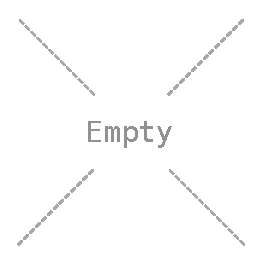
\includegraphics[height=\fgh]{empty.eps}
    }

    \mycaption{fig:eval-ms}{Mirrored \& Selective I/O performance}{Median
    sequential I/O compared to baseline. Each cluster of 3 dots between
    configurations represents the 7:3, 5:5, and 3:7 ratios as discussed in
    \cref{subsec:eval-flexible}. Distance from baseline represents overhead.}
\end{figure}
